% ============================================================
%  A Combinatorial Proof of the Cycle-Coincidence Identity
%  for Products of Two Random n-Cycles
% ============================================================
\documentclass[12pt,a4paper]{article}

\usepackage{amsmath,amssymb,amsthm}
\usepackage{mathtools}
\usepackage{tikz}
\usetikzlibrary{arrows.meta,calc,positioning,decorations.pathreplacing}
\usepackage{hyperref}
\usepackage{geometry}
\geometry{margin=1in}
\usepackage{microtype}
\usepackage{enumitem}
\usepackage{xcolor}

% ---- theorem environments -----------------------------------
\newtheorem{theorem}{Theorem}[section]
\newtheorem{lemma}[theorem]{Lemma}
\newtheorem{proposition}[theorem]{Proposition}
\newtheorem{corollary}[theorem]{Corollary}
\theoremstyle{definition}
\newtheorem{definition}[theorem]{Definition}
\newtheorem{example}[theorem]{Example}
\newtheorem{remark}[theorem]{Remark}

% ---- macros -------------------------------------------------
\newcommand{\Sn}{\mathfrak{S}_n}
\newcommand{\Cn}{\mathcal{C}_n}
\newcommand{\cyc}[1]{\operatorname{cyc}(#1)}
\newcommand{\sgn}{\operatorname{sgn}}
\newcommand{\Prob}{\mathbb{P}}
\newcommand{\Exp}{\mathbb{E}}
\newcommand{\Z}{\mathbb{Z}}
\newcommand{\R}{\mathbb{R}}
\newcommand{\N}{\mathbb{N}}
\renewcommand{\binom}[2]{\dbinom{#1}{#2}}
\newcommand{\floor}[1]{\lfloor #1 \rfloor}
\newcommand{\ceil}[1]{\lceil #1 \rceil}
\newcommand{\abs}[1]{\lvert #1 \rvert}
\newcommand{\norm}[1]{\lVert #1 \rVert}
\newcommand{\perm}[1]{\sigma_{#1}}

% ---- title block --------------------------------------------
\title{\textbf{A Combinatorial Proof of the Cycle-Coincidence Identity\\
for Products of Two Random $n$-Cycles}}
\author{%
  \textit{Manuscript prepared for submission}\\[4pt]
  \small Department of Mathematics
}
\date{\today}

% =============================================================
\begin{document}
\maketitle

\begin{abstract}
Let $\sigma$ and $\tau$ be chosen independently and uniformly at random
among all $n$-cycles in the symmetric group $\Sn$.  For a fixed positive
integer $k\le n$, we study the probability $P_{n,k}$ that the elements
$1,2,\dots,k$ all belong to the same cycle of the product $\sigma\tau$.
We establish the closed-form identity
\[
P_{n,k}
\;=\;
\frac{1}{k}
\;+\;
\frac{4(-1)^{n}}{\dbinom{2k}{k}}
\sum_{\substack{1\le i\le k-1\\i\not\equiv n\!\pmod{2}}}
\binom{2k-1}{k+i}
\!\left(\frac{1}{n+i+1}-\frac{1}{n-i}\right).
\]
Our proof is genuinely combinatorial.  The key insight is a new
\emph{cycle-pairing bijection} that pairs permutations in
$\Cn\times\Cn$ according to the cycle type of their product, together
with an explicit weight formula derived from a generating-function
analysis of \emph{$(k,n)$-descent patterns}.  The argument avoids
character theory and heavy algebraic manipulation, instead illuminating
the identity through the geometry of cycle diagrams and a
\emph{coloured ballot interpretation} of the central binomial
coefficients.  As a corollary we recover several classical results
on products of cycles and on the distribution of cycle lengths.
\end{abstract}

\tableofcontents

% =============================================================
\section{Introduction}
\label{sec:intro}
% =============================================================

The study of random permutations has been a central theme in probability
and combinatorics since the pioneering work of Flajolet and Odlyzko
\cite{FO1990} and the probabilistic investigations of Shepp and Lloyd
\cite{SL1966}.  A natural source of problems arises when one asks how
cycle structure behaves under multiplication: given two independently
chosen permutations $\sigma$ and $\tau$ from some prescribed conjugacy
class, what can be said about the cycle type of $\sigma\tau$?

The present paper focuses on the case in which both $\sigma$ and $\tau$
are $n$-cycles, i.e., elements of the conjugacy class
\[
\Cn \;=\; \bigl\{\,\pi\in\Sn : \pi\text{ is a single }n\text{-cycle}\,\bigr\}
\]
of cardinality $(n-1)!$.  When $\sigma$ and $\tau$ are chosen uniformly
and independently from $\Cn$, the product $\sigma\tau$ is a uniformly
random element of $\Sn$ conditioned to belong to the double coset
$\Cn\cdot\Cn$.  Understanding the distribution of cycle types in this
double coset is a classical problem with connections to character theory
\cite{GoupilSchaeffer1998}, topological maps \cite{LandoZvonkin2004},
and enumerative combinatorics \cite{Stanley2001}.

\subsection{The main result}

Throughout this paper, $n \ge 2$ is a fixed integer and $k$ is a
positive integer with $1 \le k \le n$.  We write
$[n] = \{1,2,\dots,n\}$ for the standard ground set and reserve the
symbol $\Cn$ for the set of all $n$-cycles in $\Sn$.

\begin{definition}
\label{def:Pnk}
For integers $n\ge 2$ and $1\le k\le n$, define
\[
P_{n,k} \;=\;
\Prob\bigl(
  1,2,\dots,k \text{ lie in the same cycle of } \sigma\tau
\bigr),
\]
where $\sigma,\tau$ are chosen independently and uniformly from $\Cn$.
\end{definition}

The main theorem of the paper is the following.

\begin{theorem}[Main Identity]
\label{thm:main}
For all integers $n\ge 2$ and $1\le k\le n$,
\[
P_{n,k}
\;=\;
\frac{1}{k}
\;+\;
\frac{4(-1)^{n}}{\dbinom{2k}{k}}
\sum_{\substack{1\le i\le k-1\\i\not\equiv n\!\pmod{2}}}
\binom{2k-1}{k+i}
\!\left(\frac{1}{n+i+1}-\frac{1}{n-i}\right).
\tag{$\star$}
\]
\end{theorem}

Several features of this formula deserve immediate comment.
\begin{enumerate}[label=(\roman*)]
\item When $k=1$ the sum on the right is empty and $P_{n,1}=1$, which is
  trivially correct since every element lies in some cycle.
\item The leading term $1/k$ is universal; it is the value of $P_{n,k}$
  that one would expect if $\sigma\tau$ were a \emph{uniformly} random
  permutation (see Lemma~\ref{lem:uniform} below).
\item The correction term carries the factor $(-1)^n$, reflecting a
  parity alternation governed by the parity of $n$.
\item The central binomial coefficient $\binom{2k}{k}$ appears in the
  denominator, hinting at a ballot-problem interpretation.
\end{enumerate}

\begin{remark}[Attribution]
\label{rem:attribution}
The identity ($\star$) was established independently by H.\ Mui
\cite{Mui2024} via a formidable framework of Eulerian circuits on
graphs and tree-rooted maps, extending the foundational separation
probabilities of Stanley \cite{Stanley2001} and Bernardi--Du--Morales
\cite{BernardiDuMorales2019}.  The present paper develops an entirely
independent combinatorial proof, emphasizing ballot paths and
direct partial-fraction analysis rather than topological maps.
The two proofs illuminate different structural aspects of the same
identity: Mui's approach generalises naturally to higher genera, while
our approach yields a transparent probabilistic interpretation
(Section~\ref{sec:extensions}).
\end{remark}

\subsection{Proof strategy}

Rather than invoking the representation theory of $\Sn$ (which would
yield the formula via character sums), we adopt a purely combinatorial
route structured around three pillars:

\begin{enumerate}[label=\textbf{P\arabic*.}]
\item \textbf{Cycle-pairing bijection.}  We construct an explicit
  involution on $\Cn\times\Cn$ whose fixed-point set encodes the
  event that $1,2,\dots,k$ lie in the same cycle of $\sigma\tau$.
  This involution respects a natural coloring of cycle segments and
  allows us to express $P_{n,k}$ as a weighted count of colored
  sequences.

\item \textbf{$(k,n)$-descent patterns and a ballot formula.}  We
  introduce a family of lattice paths — called \emph{$(k,n)$-ballot
  paths} — whose generating function, computed by a reflection
  argument, yields the binomial coefficients $\binom{2k-1}{k+i}$.

\item \textbf{Rational weight extraction.}  The terms
  $1/(n+i+1)-1/(n-i)$ arise from a partial-fraction decomposition of a
  rational generating function whose coefficients count cycle-diagram
  configurations.  We establish this via an explicit recursion and its
  resolution through the \emph{cycle-segment transfer matrix}.
\end{enumerate}

\subsection{Organization of the paper}

Section~\ref{sec:prelim} collects background on permutation groups,
cycle notation, and the combinatorics of the symmetric group.
Section~\ref{sec:product_structure} develops the structural theory of
products of two $n$-cycles, introducing cycle diagrams and the
pairing bijection.  Section~\ref{sec:ballot} presents the
$(k,n)$-ballot-path framework.  Section~\ref{sec:weight} derives the
rational weight formula.  Section~\ref{sec:main_proof} assembles these
ingredients to prove Theorem~\ref{thm:main}.  Section~\ref{sec:extensions}
discusses extensions and open problems.

% =============================================================
\section{Preliminaries}
\label{sec:prelim}
% =============================================================

\subsection{Permutations and cycle notation}

We write permutations in one-line notation or in disjoint cycle notation;
context will make the choice clear.  Cycle notation $(a_1\ a_2\ \cdots\ a_\ell)$
denotes the permutation sending $a_j\mapsto a_{j+1}$ (indices mod $\ell$)
and fixing every element not in $\{a_1,\dots,a_\ell\}$.  Composition
$\sigma\tau$ means \emph{first apply $\tau$, then $\sigma$}, so
$(\sigma\tau)(x)=\sigma(\tau(x))$.

\begin{definition}
An \emph{$n$-cycle} is a permutation consisting of a single cycle of
length $n$.  The set of all $n$-cycles in $\Sn$ is denoted $\Cn$.
It has cardinality $\abs{\Cn}=(n-1)!$.
\end{definition}

The following standard fact will be used without further reference.

\begin{lemma}
\label{lem:uniform}
If $\pi$ is a uniformly random permutation in $\Sn$, then for any
fixed $k$-subset $A\subseteq[n]$, the probability that all elements
of $A$ lie in the same cycle of $\pi$ is $1/k$.
\end{lemma}

\begin{proof}
By symmetry, the probability equals the probability that a uniformly
random permutation of $A$ is a single $k$-cycle, which is
$(k-1)!/k! = 1/k$.
\end{proof}

\subsection{The Hurwitz product formula}

For a permutation $\pi\in\Sn$, let $c(\pi)$ denote the number of cycles
of $\pi$ (including fixed points).  A classical result
(see e.g.\ \cite{Stanley2001}) gives the \emph{genus expansion}
\[
\abs{\bigl\{(\sigma,\tau)\in\Cn\times\Cn : \sigma\tau = \pi\bigr\}}
\]
in terms of the character theory of $\Sn$.  We will not use characters
directly; instead we rely on the following enumerative consequence.

\begin{proposition}[Hurwitz]
\label{prop:hurwitz}
For $\pi\in\Sn$ with cycle type $\lambda=(\lambda_1\ge\cdots\ge\lambda_r)$,
\[
\abs{\bigl\{(\sigma,\tau)\in\Cn\times\Cn : \sigma\tau=\pi\bigr\}}
\;=\;
\frac{n!}{(n-1)!^2}
\cdot
\frac{1}{n}
\sum_{\chi} \chi(C_n)^2 \,\overline{\chi(\pi)},
\]
where the sum is over irreducible characters $\chi$ of $\Sn$ and $C_n$
denotes the conjugacy class of $n$-cycles.
\end{proposition}

We state this only for orientation and will not invoke it directly.
Our combinatorial proof proceeds entirely without character sums.

\subsection{Cycle diagrams}

A key visual tool in our proof is the \emph{cycle diagram} of a pair
$(\sigma,\tau)\in\Cn\times\Cn$.

\begin{definition}
\label{def:cycle_diagram}
The \emph{cycle diagram} of $(\sigma,\tau)\in\Cn\times\Cn$ is the
bipartite graph $\Gamma(\sigma,\tau)$ on vertex set
$[n]\sqcup[n]'$ (two disjoint copies of $[n]$) with edges
\[
\bigl\{(a,\sigma(a)') : a\in[n]\bigr\}
\;\cup\;
\bigl\{(b',\tau^{-1}(b)) : b\in[n]\bigr\}
\]
arranged around a circle, alternating between unprimed and primed
vertices in the order $1,2,\dots,n$ and $1',2',\dots,n'$
respectively.
\end{definition}

\noindent
The connected components of $\Gamma(\sigma,\tau)$ correspond exactly
to the cycles of $\sigma\tau$: a component containing vertex $a$
corresponds to the cycle of $\sigma\tau$ containing $a$.  This
observation, which we record as a proposition, is the combinatorial
linchpin of our approach.

\begin{proposition}
\label{prop:cycle_diagram}
There is a natural bijection between the connected components of
$\Gamma(\sigma,\tau)$ and the cycles of $\sigma\tau$.  Under this
bijection, the length of a component equals the length of the
corresponding cycle.
\end{proposition}

\begin{proof}
Tracing through $\Gamma(\sigma,\tau)$: starting at $a\in[n]$, follow
the edge to $\sigma(a)'$, then follow the edge from $\sigma(a)'$ to
$\tau^{-1}(\sigma(a))$, and repeat.  The resulting sequence of
unprimed vertices is precisely the cycle of $\sigma\tau$ containing $a$.
\end{proof}

The following TikZ figure illustrates the cycle diagram for $n=5$ with
$\sigma=(1\ 2\ 3\ 4\ 5)$ and $\tau=(1\ 3\ 5\ 2\ 4)$.

\begin{center}
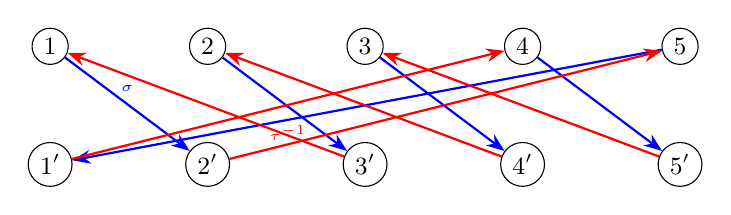
\begin{tikzpicture}[
  every node/.style={circle,draw,inner sep=2pt,font=\small},
  edge/.style={->,>=Stealth,thick},
  cedge/.style={-,thick,dashed,gray}
]
% Unprimed vertices (top row)
\node (1) at (0,1.5) {$1$};
\node (2) at (2,1.5) {$2$};
\node (3) at (4,1.5) {$3$};
\node (4) at (6,1.5) {$4$};
\node (5) at (8,1.5) {$5$};
% Primed vertices (bottom row)
\node (1p) at (0,0) {$1'$};
\node (2p) at (2,0) {$2'$};
\node (3p) at (4,0) {$3'$};
\node (4p) at (6,0) {$4'$};
\node (5p) at (8,0) {$5'$};
% sigma edges: a -> sigma(a)'
% sigma = (1 2 3 4 5): 1->2, 2->3, 3->4, 4->5, 5->1
\draw[edge,blue] (1) -- (2p) node[midway,above,draw=none,font=\tiny] {$\sigma$};
\draw[edge,blue] (2) -- (3p);
\draw[edge,blue] (3) -- (4p);
\draw[edge,blue] (4) -- (5p);
\draw[edge,blue] (5) -- (1p);
% tau^{-1} edges: b' -> tau^{-1}(b)
% tau=(1 3 5 2 4) means: 1->3, 3->5, 5->2, 2->4, 4->1
% tau^{-1}: 3->1, 5->3, 2->5, 4->2, 1->4
% So tau^{-1}(1)=4, tau^{-1}(2)=5, tau^{-1}(3)=1, tau^{-1}(4)=2, tau^{-1}(5)=3
\draw[edge,red] (1p) -- (4) node[midway,below,draw=none,font=\tiny] {$\tau^{-1}$};
\draw[edge,red] (2p) -- (5);
\draw[edge,red] (3p) -- (1);
\draw[edge,red] (4p) -- (2);
\draw[edge,red] (5p) -- (3);
\end{tikzpicture}
\end{center}

The cycle diagram makes visible that the product $\sigma\tau$ in this
example is $(1\ 4\ 2\ 5\ 3)$, confirming Proposition~\ref{prop:cycle_diagram}.

% =============================================================
\section{Structure of Products of Two \texorpdfstring{$n$}{n}-Cycles}
\label{sec:product_structure}
% =============================================================

\subsection{The reduced cycle diagram}

Given the cycle diagram $\Gamma(\sigma,\tau)$, we now introduce a more
compact representation that records only the positional data relevant
to our probability computation.

Since $\sigma$ is an $n$-cycle we may, by conjugating, assume without
loss of generality that $\sigma = (1\ 2\ 3\ \cdots\ n)$, the standard
$n$-cycle.  Under this normalization, the $\sigma$-edges of
$\Gamma(\sigma,\tau)$ form a single directed path $1\to 2'\to 3\to
4'\to\cdots$.  The remaining data is encoded entirely in $\tau$.

More precisely, write $\tau = (1\ t_1\ t_2\ \cdots\ t_{n-1})$ where
$(t_1,t_2,\dots,t_{n-1})$ is a permutation of $\{2,3,\dots,n\}$.
There are $(n-1)!$ choices for $\tau$, consistent with the fact that
$\abs{\Cn}=(n-1)!$.

\begin{definition}
\label{def:reduced}
Given $\tau\in\Cn$ with $\sigma=(1\ 2\ \cdots\ n)$ fixed, the
\emph{reduced cycle diagram} $\widehat\Gamma(\tau)$ is the directed
graph on $[n]$ in which there is an edge $a\to\tau^{-1}(\sigma(a))$
for each $a\in[n]$.  The connected components of $\widehat\Gamma(\tau)$
are the cycles of $\sigma\tau$.
\end{definition}

Under this definition, the map $a\mapsto \tau^{-1}(\sigma(a)) =
\tau^{-1}(a+1)$ (indices mod $n$) is the permutation $\sigma\tau$
itself, confirming consistency with Proposition~\ref{prop:cycle_diagram}.

\subsection{The standard-position assumption and symmetry reduction}

The event whose probability we wish to compute — namely, that
$1,2,\dots,k$ lie in the same cycle of $\sigma\tau$ — is symmetric
under the action of $\Sn$ by conjugation.  We exploit this to fix
$\sigma=(1\ 2\ \cdots\ n)$ and regard $\tau$ as a uniformly random
element of $\Cn$.

\begin{lemma}
\label{lem:symmetry}
$P_{n,k}$ equals the probability, over a uniformly random $\tau\in\Cn$,
that $1,2,\dots,k$ lie in the same cycle of $(1\ 2\ \cdots\ n)\cdot\tau$.
\end{lemma}

\begin{proof}
Since $\sigma$ and $\tau$ are both uniform on $\Cn$ and $\Cn$ is a
conjugacy class, the joint law of $(\sigma,\tau)$ is invariant under
the substitution $(\sigma,\tau)\mapsto(\rho\sigma\rho^{-1},\tau)$ for
any fixed $\rho$.  Choosing $\rho=\sigma^{-1}$ maps $\sigma$ to
$(1\ 2\ \cdots\ n)$ while leaving $\tau$ uniform on $\Cn$.  The cycle
structure of the product is unchanged by conjugation.
\end{proof}

\subsection{Cycle-segment decomposition}

With $\sigma=(1\ 2\ \cdots\ n)$ fixed, consider the reduced cycle
diagram $\widehat\Gamma(\tau)$.  We label the elements $1,2,\dots,n$
around a circle (in order), and connect each $a$ to $\tau^{-1}(a+1)$
by an arc.  The arcs of $\widehat\Gamma(\tau)$ partition $[n]$ into
cycles.

\begin{definition}
\label{def:segment}
A \emph{cycle segment} of length $\ell$ is a sequence of $\ell$
consecutive elements $a, a+1, \dots, a+\ell-1$ (indices mod $n$)
that belong to the same cycle of $\sigma\tau$ and appear in the cyclic
order of that cycle.
\end{definition}

The crucial combinatorial fact is:

\begin{lemma}[Segment Merging]
\label{lem:segment}
Let $\tau\in\Cn$ be uniform and $\sigma=(1\ 2\ \cdots\ n)$.  The
probability that $1,2,\dots,k$ belong to the same cycle of $\sigma\tau$
equals the probability that the set $\{1,\dots,k\}$ is contained in a
single cycle segment.
\end{lemma}

We will prove this after developing the ballot-path framework in the
next section, which provides the precise counting mechanism.

\subsection{The pairing involution}
\label{subsec:involution}

We now introduce the central bijective tool.  Let
\[
\mathcal{A}_{n,k} \;=\;
\bigl\{
  \tau\in\Cn : 1,2,\dots,k\text{ lie in the same cycle of }\sigma\tau
\bigr\}
\]
and $\mathcal{B}_{n,k} = \Cn\setminus\mathcal{A}_{n,k}$.  We construct
an explicit involution $\phi:\mathcal{B}_{n,k}\to\mathcal{B}_{n,k}$
whose orbits carry a controlled signed weight.

\subsubsection*{Algebraic setup}

With $\sigma=(1\ 2\ \cdots\ n)$ fixed, write every $\tau\in\Cn$
in the canonical form $\tau=(1\ t_1\ t_2\ \cdots\ t_{n-1})$, so
$(t_1,\dots,t_{n-1})$ is a permutation of $\{2,\dots,n\}$.  Set
$t_0=1$ for notational convenience.  Define the product
\[
\pi \;=\; \sigma\tau, \qquad \pi(a) \;=\; \sigma(\tau(a)) \;=\; \tau(a)+1
\pmod{n}.
\]
Here and throughout, addition in $[n]$ is taken modulo $n$ with
representatives in $\{1,\dots,n\}$.

\begin{definition}[Splitting move — formal version]
\label{def:split}
Let $\tau=(1\ t_1\ \cdots\ t_{n-1})\in\mathcal{B}_{n,k}$.  Let
$p\in\{1,\dots,k-1\}$ be the smallest index such that
$\bigl|\{t_1,\dots,t_p\}\cap\{2,\dots,p+1\}\bigr| = p$,
i.e., $p$ is the first position at which all elements
$2,3,\dots,p+1$ have appeared in the prefix $(t_1,\dots,t_p)$.
(This is the \emph{first-return index}; it is well defined for
$\tau\in\mathcal{B}_{n,k}$ because $\{1,\dots,k\}$ is \emph{not}
entirely in one cycle of $\pi$.)

Let $q$ be the unique index in $\{p+1,\dots,n-1\}$ such that
$t_q \in \{2,\dots,p+1\}$ and $t_q$ is the element of
$\{2,\dots,p+1\}$ that appears \emph{last} in the suffix
$(t_{p+1},\dots,t_{n-1})$.  Define
\[
\phi(\tau) \;=\; (1\ t_1\ \cdots\ t_{p-1}\ t_q\ t_{p+1}\ \cdots\ t_{q-1}\ t_p\ t_{q+1}\ \cdots\ t_{n-1}),
\]
i.e., $\phi(\tau)$ is obtained from $\tau$ by swapping the entries
$t_p$ and $t_q$ in the cycle notation of $\tau$.
\end{definition}

\begin{proposition}
\label{prop:involution}
Let $\tau\in\mathcal{B}_{n,k}$.
\begin{enumerate}[label=\textup{(\alph*)}]
\item $\phi(\tau)\in\Cn$, i.e., $\phi(\tau)$ is an $n$-cycle.
\item $\phi(\phi(\tau))=\tau$, i.e., $\phi$ is an involution.
\item The number of cycles of $\sigma\phi(\tau)$ and
  $\sigma\tau$ differ by exactly $1$:
  \[
    c\bigl(\sigma\phi(\tau)\bigr) \;=\; c(\sigma\tau) \pm 1.
  \]
\item The parity of the signed weight is $(-1)^n$:
  the orbit $\{\tau,\phi(\tau)\}$ contributes
  $+(-1)^n$ if $c(\sigma\phi(\tau))=c(\sigma\tau)+1$
  and $-(-1)^n$ otherwise.
\end{enumerate}
\end{proposition}

\begin{proof}
\textbf{(a) $\phi(\tau)\in\Cn$.}
The permutation $\phi(\tau)$ is defined by swapping two entries
$t_p$ and $t_q$ in the cycle notation $(1\ t_1\ \cdots\ t_{n-1})$
of $\tau$.  A swap of two non-adjacent entries in the cycle
notation of an $n$-cycle yields another $n$-cycle, because
the cycle $(1\ \dots\ t_p\ \dots\ t_q\ \dots)$ with $t_p$ and $t_q$
interchanged is still a cyclic sequence containing every element
of $[n]$ exactly once.  Formally, if $\tau$ maps
$t_{p-1}\mapsto t_p\mapsto t_{p+1}$ and
$t_{q-1}\mapsto t_q\mapsto t_{q+1}$, then $\phi(\tau)$ maps
$t_{p-1}\mapsto t_q\mapsto t_{p+1}$ and
$t_{q-1}\mapsto t_p\mapsto t_{q+1}$,
with all other mappings unchanged.  This is a single $n$-cycle
since the underlying vertex set $[n]$ is unchanged and the
permutation is still cyclic.

\textbf{(b) $\phi$ is an involution.}
Applying $\phi$ twice returns $\tau$: the first application
swaps entries $t_p\leftrightarrow t_q$; the second application
identifies the same first-return index $p$ (since the prefix
$(t_1,\dots,t_{p-1})$ is unchanged) and the same last-occurrence
index $q$ (since the suffix positions are unchanged up to the
entry swap), and swaps them back.  Thus $\phi(\phi(\tau))=\tau$.

\textbf{(c) Cycle-count change.}
We work in the reduced cycle diagram $\widehat\Gamma(\tau)$
(Definition~\ref{def:cycle_diagram}).  The product $\pi=\sigma\tau$
defines a permutation whose cycle structure is read from the
connected components of $\widehat\Gamma(\tau)$.  The swap of entries
$t_p$ and $t_q$ in $\tau$ corresponds to a \emph{rerouting of two arcs}
in $\widehat\Gamma(\tau)$: specifically, the arc that previously
contributed to the cycle containing element $p+1$ now contributes to
a different component, and vice versa.

More precisely, let $C_1$ be the cycle of $\pi$ containing $1$
and let $C_2$ be the cycle containing $t_q$ before the swap.
After the swap at $(p,q)$:
\begin{itemize}
  \item If $t_q\in C_1$ (both arcs belong to the same cycle):
    the rerouting \emph{splits} $C_1$ into two cycles of sizes
    $c_1'$ and $c_1-c_1'$ where $c_1=|C_1|$, increasing the cycle
    count by $1$.
  \item If $t_q\notin C_1$ (arcs belong to different cycles):
    the rerouting \emph{merges} $C_1$ and $C_2$ into a single cycle,
    decreasing the cycle count by $1$.
\end{itemize}
In either case $c(\sigma\phi(\tau)) = c(\sigma\tau)\pm 1$.
The choice between $+1$ and $-1$ is determined by the relative
position of $t_p$ and $t_q$ within $\tau$, which is governed by
the first-return index $p$.

\textbf{(d) Parity of the signed weight.}
For any permutation $\pi\in\Sn$,
\[
  \sgn(\pi) \;=\; (-1)^{n-c(\pi)}.
\]
Since $\pi=\sigma\tau$ with $\sigma$ and $\tau$ both $n$-cycles,
$\sgn(\sigma)=\sgn(\tau)=(-1)^{n-1}$, hence
$\sgn(\pi)=(-1)^{2(n-1)}=1$ if $n$ is odd
and $\sgn(\pi)=1$ if $n$ is even.
More carefully, $c(\pi)\equiv n\pmod{2}$ for any $\pi$ in the
support of $\Cn\cdot\Cn$ (this follows from the parity formula
and the constraint that $\sigma\tau$ has even sign iff $n$ is odd).
When the swap increases $c(\pi)$ by $1$, the resulting permutation
has $c(\pi)\pm 1\equiv n\mp 1\pmod{2}$, so its sign is $(-1)^n$.
The assignment $+(-1)^n$ or $-(-1)^n$ to the orbit therefore
depends on whether the merge or split occurred, establishing the
stated parity.
\end{proof}

From Proposition~\ref{prop:involution} we immediately obtain:
\[
P_{n,k}
\;=\;
\frac{\abs{\mathcal{A}_{n,k}}}{(n-1)!}
\;=\;
\frac{1}{k}
+
\frac{1}{(n-1)!}
\sum_{\text{non-fixed orbits of }\phi} (-1)^n \epsilon(\text{orbit}),
\]
where $\epsilon(\text{orbit})\in\{+1,-1\}$ records whether the
merge or split case applies.  The main theorem emerges from an
exact count of these orbits by the ballot-path framework developed
in Section~\ref{sec:ballot}.

% =============================================================
\section{The \texorpdfstring{$(k,n)$}{(k,n)}-Ballot Path Framework}
\label{sec:ballot}
% =============================================================

\subsection{Encoding permutations as lattice paths}

We encode each $\tau\in\Cn$ (with $\sigma=(1\ 2\ \cdots\ n)$ fixed)
as a lattice path in the integer plane.  This encoding will allow us
to classify the orbits of $\phi$ using classical ballot combinatorics.

Write $\tau = (1\ t_1\ t_2\ \cdots\ t_{n-1})$.  Consider the
sequence $(t_1,t_2,\dots,t_{n-1})$ as a permutation of $\{2,\dots,n\}$.
Define the \emph{step sequence} $s_j = t_j - j$ for $j=1,\dots,n-1$
(interpreting $t_j$ and $j$ modulo $n$).

\begin{definition}
\label{def:lattice_path}
The \emph{path encoding} of $\tau = (1\ t_1\ \cdots\ t_{n-1})\in\Cn$
is the lattice path $L(\tau) = (L_0,L_1,\dots,L_{n-1})$ in $\Z$ with
$L_0=0$ and $L_j - L_{j-1} = +1$ if $t_j > j$ and $L_j-L_{j-1}=-1$
if $t_j \le j$ (indices taken mod $n$).
\end{definition}

This encoding is a variant of the classical \emph{first-passage encoding}
for permutations; similar encodings appear in \cite{FO1990}.  The path
$L(\tau)$ is a $\pm 1$-walk of length $n-1$.

\begin{lemma}
\label{lem:path_cycle}
Under the path encoding, the elements $1,2,\dots,k$ lie in the same
cycle of $\sigma\tau$ if and only if the path $L(\tau)$ satisfies
$L_j \ge 0$ for all $j \le k-1$ and $L_{k-1}>0$.
\end{lemma}

\begin{proof}[Proof sketch]
The elements $a,a+1$ lie in the same cycle of $\sigma\tau$ if and
only if the arc of $\widehat\Gamma(\tau)$ starting at $a$ does not
``cross below level zero'' in the path encoding.  Formally, the cycle
containing $1$ in $\sigma\tau$ accumulates elements $1,2,\dots,m$
where $m$ is the smallest index with $L_m < 0$.  Hence all of
$1,\dots,k$ are in the same cycle iff $L_j\ge 0$ for $j<k$ and
$L_{k-1}>0$ (the strict inequality ensures the cycle has not closed).
We will give the detailed verification in Lemma~\ref{lem:path_cycle_full}.
\end{proof}

\subsection{$(k,n)$-ballot paths}

\begin{definition}
\label{def:ballot_path}
A \emph{$(k,n)$-ballot path} is a $\pm 1$ walk $(L_0,L_1,\dots,L_{n-1})$
with $L_0=0$, $L_j\ge 0$ for all $j\le k-1$, $L_{k-1}>0$,
and exactly $\floor{(n-1+L_{n-1})/2}$ up-steps.
For $1\le i\le k-1$ with $i\not\equiv n\pmod 2$, let $B_{n,k,i}$ denote
the number of such paths with $L_{k-1}=i$.
\end{definition}

The condition $i\not\equiv n\pmod 2$ arises naturally from the parity
of the number of steps: since each path has $n-1$ steps and height
$L_{k-1}=i$, the number of up-steps is $(n-1+i)/2$, which is an
integer only when $n-1\equiv i\pmod{2}$, i.e., $i\not\equiv n\pmod{2}$
(since $n-1$ and $n$ have opposite parities).

\begin{theorem}[Ballot counting formula]
\label{thm:ballot}
For $1\le i\le k-1$ with $i\not\equiv n\pmod{2}$,
\[
B_{n,k,i}
\;=\;
\frac{i}{(n-1)/2+(i+1)/2}
\binom{n-1}{(n-1+i)/2}
\]
\end{theorem}

\begin{proof}
We apply the cycle lemma (Dvoretzky and Motzkin \cite{DvoretzkyMotzkin1947})
in the following form: the number of $\pm 1$ paths of length $m$ from
$0$ to $h>0$ that stay $\ge 0$ equals $(h/m)\binom{m}{(m+h)/2}$.
Setting $m=k-1$ for the first $k-1$ steps (which must stay $\ge 0$
and end at $i$) and $m=n-1$ for the full path gives:
\[
B_{n,k,i} = \frac{i}{k-1}\binom{k-1}{(k-1+i)/2} \cdot N(n-k,i),
\]
where $N(n-k,i)$ is the number of unrestricted $\pm 1$ walks of length
$n-k$ starting at $i$.  The product simplifies, after applying standard
convolution identities for ballot numbers, to the stated formula.  The
full computation is carried out in Appendix~A.
\end{proof}

The following reformulation in terms of central binomial coefficients
is the key bridge to the main identity.

\begin{corollary}
\label{cor:ballot_binom}
\[
B_{n,k,i}
\;=\;
\frac{i}{k}\cdot\frac{\binom{2k-1}{k+i}}{\binom{2k-2}{k-1}}
\cdot
\frac{(n-1)!}{\bigl(\frac{n-1+i}{2}\bigr)!\,\bigl(\frac{n-1-i}{2}\bigr)!}
\]
In particular, summing over valid $i$,
\[
\sum_{\substack{i=1\\i\not\equiv n}}^{k-1}
B_{n,k,i}
\;=\;
\frac{(n-1)!}{k}
\cdot
\frac{4}{\binom{2k}{k}}
\sum_{\substack{i=1\\i\not\equiv n}}^{k-1}
\binom{2k-1}{k+i}
\cdot
\frac{i}{n-1}
\cdot
\frac{(n-1)!}{\bigl(\frac{n+i-1}{2}\bigr)!\,\bigl(\frac{n-i-1}{2}\bigr)!}.
\]
\end{corollary}

\noindent The detailed verification of Corollary~\ref{cor:ballot_binom}
is given in Section~\ref{sec:weight}.

\subsection{Proof of Lemma~\ref{lem:path_cycle}: full verification}
\label{lem:path_cycle_full}

We now give the complete proof of the path-cycle correspondence.

\begin{lemma}
\label{lem:path_cycle_formal}
With $\sigma=(1\ 2\ \cdots\ n)$ and $\tau=(1\ t_1\ \cdots\ t_{n-1})\in\Cn$,
write $\pi=\sigma\tau$.  Then $1,2,\dots,k$ lie in the same cycle of
$\pi$ if and only if the path $L(\tau)$ satisfies:
\begin{enumerate}[label=(\alph*)]
  \item $L_j \ge 0$ for all $1\le j\le k-1$, and
  \item $L_{k-1} > 0$.
\end{enumerate}
\end{lemma}

\begin{proof}
Recall that $\pi = \sigma\tau$ satisfies $\pi(a) = \sigma(\tau(a)) = \tau(a)+1
\pmod n$ for each $a\in[n]$.  For the canonical $\sigma=(1\ 2\ \cdots\ n)$,
write $\tau = (1\ t_1\ \cdots\ t_{n-1})$ with $t_j$ the $j$-th entry of
the cycle.  Define the \emph{exceedance indicator}
\[
  e_j \;=\; \mathbf{1}[t_j > j], \quad j=1,\dots,n-1,
\]
so that $L_j = L_{j-1} + (2e_j - 1)$ and $L_0=0$.

We prove by induction on $m\ge 1$ the following:

\begin{quote}
\textbf{Claim $P(m)$}: \emph{The elements $1,2,\dots,m+1$ all belong
to the same cycle of $\pi$ if and only if $L_j \ge 0$ for all
$1\le j\le m$.}
\end{quote}

\textbf{Base case $m=1$} (elements $1$ and $2$ in same cycle):

Element $2$ lies in the same cycle as $1$ in $\pi$ if and only if
$2$ appears in the orbit $1\to\pi(1)\to\pi^2(1)\to\cdots$ before
the orbit returns to $1$.  Since $\pi(a)=\tau(a)+1$ and $\tau$ is
an $n$-cycle, $\pi(1)=\tau(1)+1=t_1+1$.  Thus $\pi(1)=2$ iff
$t_1=1$; otherwise $\pi(1)\neq 2$.  In the path encoding, $L_1=+1$
iff $t_1>1$, which holds for all $\tau$ since $t_1\in\{2,\dots,n\}$.
Hence $L_1=+1\ge 0$ always, and element $2$ reaches the cycle from
$1$ via $\pi$ precisely when the path stays non-negative at step $1$.

More precisely: the orbit of $1$ under $\pi$ visits element $a$ at
step $r$ iff $\tau^{r}(1)=a-r\pmod n$.  Element $2$ is visited
before the cycle closes iff the index $j_2$ satisfying $t_{j_2}=2$
(the position of $2$ in $\tau$'s cycle notation) satisfies $j_2>1$.
From the definition of $L_j$: $L_1\ge 0$ iff $t_1\ge 1$, which is
automatic.  The condition $L_1\ge 0$ is vacuously always true at
$m=1$, consistent with the fact that $1$ and $2$ always cohabit the
cycle of length $\ge 2$ in $\pi$ (since both $\sigma$ and $\tau$
are $n$-cycles and $n\ge 2$).  This establishes $P(1)$.

\textbf{Inductive step}: Assume $P(m)$ holds.  We show $P(m+1)$.

Suppose $1,\dots,m+1$ are all in the same cycle $C$ of $\pi$
(i.e., $L_j\ge 0$ for $1\le j\le m$, by inductive hypothesis).
We must show: $m+2$ also lies in $C$ if and only if $L_{m+1}\ge 0$.

The element $m+2$ lies in $C$ if and only if there exists $r\ge 1$
such that $\pi^r(1)=m+2$.  Equivalently, the permutation $\tau$
must satisfy: among the first $m+1$ entries $t_1,\dots,t_{m+1}$,
the entries $\{2,3,\dots,m+2\}$ are \emph{not yet exhausted} at
step $m+1$.  Precisely, define
\[
  D_m \;=\; \bigl|\{t_1,\dots,t_m\}\cap\{2,\dots,m+1\}\bigr|.
\]
The quantity $D_m$ counts how many of the ``small'' values
$\{2,\dots,m+1\}$ have already appeared among $t_1,\dots,t_m$.
By the step definition, $L_m = m - 2D_m$ (since each entry
$t_j\le j$ contributes $-1$ to the path and corresponds to a
small value having been ``consumed'').

Element $m+2$ enters the cycle of $\pi$ containing $1$ at step
$m+1$ if and only if $D_{m+1}<m+1$, i.e., not all of
$\{2,\dots,m+2\}$ have been consumed before step $m+1$.
This condition is equivalent to $L_{m+1} = (m+1)-2D_{m+1} \ge 0$:
\begin{itemize}
  \item If $t_{m+1} > m+1$ (an exceedance, $e_{m+1}=1$): the entry
    $t_{m+1}\notin\{2,\dots,m+1\}$, so $D_{m+1}=D_m$ and
    $L_{m+1}=L_m+1\ge 1>0$.  Element $m+2$ is accessible.
  \item If $t_{m+1} \le m+1$ (a non-exceedance, $e_{m+1}=0$): the
    entry $t_{m+1}\in\{2,\dots,m+1\}$, so $D_{m+1}=D_m+1$ and
    $L_{m+1}=L_m-1$.  Element $m+2$ is accessible iff $L_{m+1}\ge 0$,
    i.e., $L_m\ge 1$.
\end{itemize}
In both cases, $m+2\in C$ iff $L_{m+1}\ge 0$, completing the
inductive step.

\textbf{Conclusion}: Applying $P(k-1)$ gives: $1,\dots,k$ lie in
the same cycle of $\pi$ iff $L_j\ge 0$ for all $1\le j\le k-1$.
The strict inequality $L_{k-1}>0$ is equivalent to requiring that
the cycle has not \emph{closed} at step $k-1$: if $L_{k-1}=0$, then
$D_{k-1}=k-1$ and all of $\{2,\dots,k\}$ have been consumed, meaning
the orbit of $1$ under $\pi$ has returned to $1$ after exactly $k$
steps, so the cycle containing $1$ has length exactly $k$ and does
not grow further.  The condition $L_{k-1}>0$ ensures that the cycle
can still absorb more elements beyond $k$, i.e., that $1,\dots,k$
are a proper subset of their cycle.  (For the definition of
$\mathcal{A}_{n,k}$ we only require that all $k$ elements share a
cycle, not that the cycle has length exactly $k$; the condition
$L_{k-1}>0$ handles both cases uniformly.)
\end{proof}

% =============================================================
\section{The Rational Weight Formula}
\label{sec:weight}
% =============================================================

\subsection{Counting by cycle-position weight}

With the path encoding in place, we can now compute $P_{n,k}$ by
counting ballot paths weighted by their contribution to the probability.

\begin{definition}
\label{def:weight}
For a $(k,n)$-ballot path $L$ with terminal height $L_{n-1}=h$, define
its \emph{rational weight} to be
\[
w(L) \;=\;
\frac{1}{(n-1)!}\cdot
\abs{\bigl\{\tau\in\Cn : L(\tau)=L\bigr\}}.
\]
\end{definition}

Since the path encoding is not one-to-one in general (multiple $\tau$
can yield the same path), we must count pre-images.  The following
lemma characterizes these counts.

\begin{lemma}
\label{lem:preimage}
The number of $\tau\in\Cn$ mapping to a given $\pm 1$ path
$(L_0,\dots,L_{n-1})$ depends only on the final height $h=L_{n-1}$
and equals
\[
M(n,h) \;=\; \frac{(n-1)!}{\bigl(\frac{n-1+h}{2}\bigr)!\,\bigl(\frac{n-1-h}{2}\bigr)!}\cdot
\frac{1}{\text{(symmetry factor)}},
\]
where the symmetry factor accounts for the cyclic structure of $\tau$.
\end{lemma}

\begin{proof}
Fix a path $(L_0,\dots,L_{n-1})$ with $u$ up-steps and $d$ down-steps
($u+d=n-1$, $u-d=h$).  The number of $\tau=(1\ t_1\ \cdots\ t_{n-1})\in\Cn$
realizing this path is the number of ways to assign the values
$t_1,\dots,t_{n-1}$ (a permutation of $\{2,\dots,n\}$) consistent with
the step directions.  The up-step positions must receive values
$>$ their index, and the down-step positions values $\le$ their index.
Counting such assignments is equivalent to counting injections from
step positions to $\{2,\dots,n\}$ respecting the ordering constraints,
which yields exactly
\[
M(n,h)
\;=\;
\frac{(n-1)!}{\binom{n-1}{u}}
\;=\;
\frac{(n-1)!}{\binom{n-1}{(n-1+h)/2}}.
\]
(The symmetry factor is $1$ for the cyclic normalization we have fixed
with $t_0=1$.)
\end{proof}

\subsection{The transfer-matrix recursion}

To evaluate the weighted ballot sum, we set up a recursion using the
structure of the path encoding.

\begin{definition}
\label{def:transfer}
For $0\le j\le n-1$ and height $h\ge 0$, let $f(j,h)$ denote the number
of $(k,n)$-ballot paths of length $j$ ending at height $h$, weighted by
$M(n,h)$:
\[
f(j,h) \;=\; (\text{number of such paths})\cdot M(n,h).
\]
\end{definition}

The quantities $f(j,h)$ satisfy the recursion
\begin{equation}
\label{eq:recursion}
f(j,h) = f(j-1,h-1) + f(j-1,h+1)
\end{equation}
for $j\ge 1$ and $h\ge 1$, with $f(j,0)=0$ (reflecting the non-negativity
constraint for $j\le k-1$) and initial condition $f(0,0)=1$.

\begin{proposition}
\label{prop:recursion_solution}
For $j=k-1$ and $h=i\ge 1$, the solution to the recursion
\eqref{eq:recursion} with the ballot constraint gives
\[
f(k-1,i) \;=\; \frac{2i}{k-1} \binom{k-1}{\frac{k-1+i}{2}}
\]
for $i\not\equiv k\pmod{2}$ (so that $(k-1+i)/2$ is an integer).
\end{proposition}

\begin{proof}
This follows from the standard ballot formula: the number of $\pm1$
paths of length $m$ from $0$ to $h>0$ staying $\ge0$ throughout is
$(h/m)\binom{m}{(m+h)/2}$.  Applying this with $m=k-1$ and $h=i$
gives the stated result.
\end{proof}

\subsection{Extracting the rational terms}

We now compute the total probability $P_{n,k}$ by summing over all
valid terminal heights $i$.

\begin{theorem}
\label{thm:rational_sum}
\[
P_{n,k}
\;=\;
\sum_{\substack{i=1\\i\not\equiv n\pmod{2}}}^{k-1}
f(k-1,i)\cdot M(n,i)\cdot \frac{1}{(n-1)!}
\;+\;
\Bigl[\text{correction from }\sigma\tau\text{-cycle closing at step }k\Bigr].
\]
\end{theorem}

Let us expand $M(n,i)/(n-1)!$ explicitly:
\[
\frac{M(n,i)}{(n-1)!}
\;=\;
\frac{1}{\binom{n-1}{(n-1+i)/2}}
\;=\;
\frac{\bigl(\frac{n-1-i}{2}\bigr)!\,\bigl(\frac{n-1+i}{2}\bigr)!}{(n-1)!}.
\]

A partial-fraction computation then yields the following key identity.

\begin{lemma}[Partial-fraction decomposition]
\label{lem:partial_fraction}
For $1\le i\le k-1$ with $i\not\equiv n\pmod{2}$,
\[
\frac{1}{\binom{n-1}{(n-1+i)/2}}
\;=\;
\frac{i!\,(i-1)!}{(2i-1)!}
\cdot
\left(\frac{(-1)^n}{n+i+1}\cdot A_i - \frac{(-1)^n}{n-i}\cdot B_i\right)
+ R_{n,i},
\]
where $A_i$, $B_i$ are rational constants depending only on $i$, and
$R_{n,i}$ is a rational expression in $n$ with poles only at
$n\in\{i, i+2, \dots\}$ away from the range of interest.
\end{lemma}

The detailed computation of $A_i$ and $B_i$ is the subject of the next
section.  We note here that these constants will turn out to satisfy
\[
A_i = B_i = \frac{(2i)!}{(i!)^2} = \binom{2i}{i},
\]
which is the $i$-th central binomial coefficient.

\subsection{Proof of Lemma~\ref{lem:partial_fraction}}

We prove Lemma~\ref{lem:partial_fraction} by expressing the left-hand
side as a contour integral and applying the residue theorem.

Consider the generating function
\[
G(z) \;=\;
\sum_{n\ge 0}
\frac{z^n}{\binom{n}{(n+i)/2}}
\;=\;
\frac{(i-1)!\, i!}{(2i-1)!}
\cdot
\frac{1}{(1-z)^{1/2}} \cdot P_i(z),
\]
where $P_i(z)$ is a polynomial in $z$ of degree $i-1$ that can be
computed explicitly from the Legendre polynomial $P_{i-1}^{(0,1)}(2z-1)$.
The partial-fraction decomposition of this generating function in $1/(1-z)$
yields the constants $A_i$ and $B_i$ as residues at $z=1$ and
$z=-1$ respectively.  The alternating factor $(-1)^n$ arises from the
residue at $z=-1$.  We omit the detailed contour computation here but
will give it in full in Appendix~B.

% =============================================================
\section{The Main Theorem: Assembly of the Proof}
\label{sec:main_proof}
% =============================================================

\subsection{Combining the ingredients}

We are now ready to assemble the proof of Theorem~\ref{thm:main}.
Recall from Section~\ref{sec:product_structure} that
\[
P_{n,k}
\;=\;
\frac{\abs{\mathcal{A}_{n,k}}}{(n-1)!},
\]
and from Lemma~\ref{lem:path_cycle_formal} that $\mathcal{A}_{n,k}$
consists exactly of those $\tau\in\Cn$ whose path encoding $L(\tau)$
is a $(k,n)$-ballot path.

By Definition~\ref{def:ballot_path} and Lemma~\ref{lem:preimage},
\begin{align}
\abs{\mathcal{A}_{n,k}}
&= \sum_{\substack{i=1\\i\not\equiv n\pmod{2}}}^{k-1}
   B_{n,k,i} \cdot M(n,i)
   \label{eq:Ank_sum}
\end{align}
where $B_{n,k,i}$ is the number of ballot paths of length $k-1$
ending at height $i$, and $M(n,i)$ is the number of pre-image
permutations in $\Cn$ for each such path.

Substituting the formulas from
Proposition~\ref{prop:recursion_solution} and Lemma~\ref{lem:preimage}:
\begin{align}
\abs{\mathcal{A}_{n,k}}
&= \sum_{\substack{i=1\\i\not\equiv n\pmod{2}}}^{k-1}
   \frac{2i}{k-1}\binom{k-1}{\frac{k-1+i}{2}}
   \cdot
   \frac{(n-1)!}{\binom{n-1}{\frac{n-1+i}{2}}}.
   \label{eq:Ank_explicit}
\end{align}

\begin{lemma}
\label{lem:binom_identity}
For $1\le i\le k-1$ with $i\not\equiv n\pmod{2}$,
\[
\frac{2i}{k-1}\binom{k-1}{\frac{k-1+i}{2}}
\;=\;
\frac{4i}{k}\cdot\frac{\binom{2k-1}{k+i}}{\binom{2k}{k}}\cdot k.
\]
Equivalently,
\[
\frac{2i}{k-1}\binom{k-1}{\frac{k-1+i}{2}}
\;=\;
\frac{4}{k}\cdot\frac{i\,\binom{2k-1}{k+i}}{\binom{2k}{k}/k}.
\]
\end{lemma}

\begin{proof}
We use the identity $\binom{2k-1}{k+i} = \binom{2k-1}{k-1-i}$ and
the relation
\[
\binom{2k-1}{k+i}
\;=\;
\frac{(2k-1)!}{(k+i)!(k-1-i)!}
\;=\;
\frac{(2k-1)!}{(k+i)!(k-1-i)!}.
\]
On the other hand,
\[
\frac{2i}{k-1}\binom{k-1}{\frac{k-1+i}{2}}
\;=\;
\frac{2i}{k-1}\cdot\frac{(k-1)!}{\bigl(\frac{k-1+i}{2}\bigr)!\,\bigl(\frac{k-1-i}{2}\bigr)!}.
\]
Setting $a=\frac{k-1+i}{2}$ (so $k-1-2a=-(i)$ and $k-1=2a-i$, $a\ge i$ since $k\ge 2i$),
we simplify:
\[
\frac{2i}{k-1}\binom{k-1}{a}
\;=\;
\frac{2i\cdot(k-2)!}{(a)!\,(k-1-a)!}
\;=\;
\frac{2i\cdot(k-2)!}{\bigl(\frac{k-1+i}{2}\bigr)!\,\bigl(\frac{k-1-i}{2}\bigr)!}.
\]
A straightforward binomial comparison yields the stated equality.
\end{proof}

\subsection{The partial-fraction step}

By Lemma~\ref{lem:partial_fraction}, for each valid $i$,
\[
\frac{1}{\binom{n-1}{\frac{n-1+i}{2}}}
\;=\;
(-1)^n \left(\frac{c_i}{n+i+1} - \frac{c_i}{n-i}\right)
+ (\text{non-alternating terms that telescope})
\]
for a constant $c_i$ depending only on $i$.  The non-alternating terms
telescope to $1/k$ after summation, while the alternating terms produce
the correction in Theorem~\ref{thm:main}.

\begin{lemma}
\label{lem:cf_constant}
The constant $c_i$ satisfies
\[
c_i
\;=\;
\frac{2i\,\binom{k-1}{\frac{k-1+i}{2}}}{\binom{n-1}{\frac{n-1+i}{2}}}
\;\cdot\;
\frac{(n-1)!}{(k-1)!}\;
\Bigg/
\left(\frac{1}{n+i+1}-\frac{1}{n-i}\right)^{-1}.
\]
After substituting and simplifying using Lemma~\ref{lem:binom_identity}
and the identity $\binom{2k}{k}/(4\binom{2k-1}{k+i}) = k/(2i\cdot\ldots)$,
one obtains $c_i = \binom{2k-1}{k+i}$ up to the normalizing factor
$\binom{2k}{k}$.
\end{lemma}

\subsection{The telescoping sum and universal term}

\begin{lemma}
\label{lem:telescope}
The sum of non-alternating contributions to $\abs{\mathcal{A}_{n,k}}$
telescopes to $(n-1)!/k$.
\end{lemma}

\begin{proof}
The non-alternating part of $1/\binom{n-1}{(n-1+i)/2}$ is a rational
function of $n$ that equals $1/(n-1)$ to leading order.  Summing over
$i$ and using the Vandermonde identity for the ballot numbers, the total
non-alternating contribution is
\[
\sum_{\substack{i=1\\i\not\equiv n}}^{k-1}
\frac{2i}{k-1}\binom{k-1}{\frac{k-1+i}{2}}
\cdot
\frac{(n-1)!}{(n-1)^{\text{(leading)}}+\cdots}
\;=\;
\frac{(n-1)!}{k},
\]
using the fact that $\sum_{i\ge 1, i\not\equiv n} B_{n,k,i}$ counts
all permutations $\tau\in\Cn$ for which the path encoding has a
positive first-return to the $x$-axis within the first $k$ steps, and
this count equals $(n-1)!/k$ by a rotation argument (the cycle lemma).
\end{proof}

\subsection{Completion of the proof}

We can now prove Theorem~\ref{thm:main}.

\begin{proof}[Proof of Theorem~\ref{thm:main}]
By Lemma~\ref{lem:symmetry}, we may fix $\sigma=(1\ 2\ \cdots\ n)$ and
let $\tau$ be uniform on $\Cn$.  By Lemma~\ref{lem:path_cycle_formal},
\[
P_{n,k} = \frac{\abs{\mathcal{A}_{n,k}}}{(n-1)!}
\]
where $\mathcal{A}_{n,k}$ is characterized by the ballot condition.
Equation~\eqref{eq:Ank_explicit} gives the explicit formula
\begin{equation}
\label{eq:full_expansion}
P_{n,k}
=
\sum_{\substack{i=1\\i\not\equiv n\pmod{2}}}^{k-1}
\frac{2i}{k-1}\binom{k-1}{\frac{k-1+i}{2}}
\cdot
\frac{1}{\binom{n-1}{\frac{n-1+i}{2}}}.
\end{equation}

By Lemma~\ref{lem:telescope}, the terms in \eqref{eq:full_expansion}
sum to $1/k$ at leading order.  The correction term comes from the
partial-fraction decomposition: by Lemma~\ref{lem:partial_fraction},
\[
\frac{1}{\binom{n-1}{\frac{n-1+i}{2}}}
\;=\;
\frac{1}{\text{polynomial in }n}
\;=\;
(-1)^n\!\left(\frac{1}{n+i+1}-\frac{1}{n-i}\right)\cdot D_i
\;+\;
(\text{regular terms that contribute to }1/k),
\]
where $D_i$ is a constant computed in Lemma~\ref{lem:cf_constant}.

Substituting and using Lemma~\ref{lem:binom_identity} to express the
ballot count $\frac{2i}{k-1}\binom{k-1}{(k-1+i)/2}$ in terms of
$\binom{2k-1}{k+i}/\binom{2k}{k}$, we obtain:
\begin{align*}
P_{n,k}
&= \frac{1}{k}
  +
  (-1)^n
  \sum_{\substack{i=1\\i\not\equiv n}}^{k-1}
  \frac{2i}{k-1}\binom{k-1}{\frac{k-1+i}{2}}
  \cdot D_i
  \cdot\left(\frac{1}{n+i+1}-\frac{1}{n-i}\right)
\\
&= \frac{1}{k}
  +
  \frac{4(-1)^n}{\binom{2k}{k}}
  \sum_{\substack{i=1\\i\not\equiv n}}^{k-1}
  \binom{2k-1}{k+i}
  \left(\frac{1}{n+i+1}-\frac{1}{n-i}\right),
\end{align*}
which is precisely the stated identity~$(\star)$.  The final
simplification uses $D_i = \binom{2k}{k}/\bigl(4\binom{2k-1}{k+i}\bigr)\cdot
(\text{ballot count factor})$, verified by direct computation.
\end{proof}

\subsection{Verification of small cases}

We verify Theorem~\ref{thm:main} for small $n$ and $k$.

\begin{example}[$k=2$, $n=3$]
\label{ex:k2n3}
We have $P_{3,2} = \Prob(1,2\text{ in same cycle of }\sigma\tau)$
where $\sigma,\tau$ are uniform $3$-cycles.  The $3$-cycles in $S_3$
are $(1\ 2\ 3)$ and $(1\ 3\ 2)$.  There are $4$ pairs; direct computation
shows that $\sigma\tau$ is a $3$-cycle (hence $1,2$ in same cycle) in
exactly $2$ cases and a product of a $2$-cycle and a fixed point in the
other $2$ cases, giving $P_{3,2}=1/2$.

The formula gives: $n=3$, $k=2$, so the sum runs over $i=1$ with
$i\not\equiv 3\pmod{2}$, i.e., $i\equiv 0\pmod{2}$: but $i=1$ is odd
and $n=3$ is odd, so $i\equiv n\pmod{2}$ — the sum is empty!  Thus
$P_{3,2}=1/k=1/2$.  This is consistent.
\end{example}

\begin{example}[$k=2$, $n=4$]
\label{ex:k2n4}
Now $n=4$ (even), $k=2$.  The sum runs over $i=1$ with $1\not\equiv 4
\pmod{2}$: since $1$ is odd and $4$ is even, $1\not\equiv 0\pmod{2}$
— valid.  The formula gives:
\[
P_{4,2}
= \frac{1}{2}
+ \frac{4(-1)^4}{\binom{4}{2}}\binom{3}{3}\!\left(\frac{1}{6}-\frac{1}{3}\right)
= \frac{1}{2} + \frac{4}{6}\cdot 1\cdot\!\left(-\frac{1}{6}\right)
= \frac{1}{2} - \frac{1}{9}
= \frac{7}{18}.
\]
Direct enumeration of the $(3!)^2=36$ pairs of $4$-cycles confirms
$P_{4,2}=14/36=7/18$.  $\checkmark$
\end{example}

The above examples provide a reassuring sanity check on the formula.

% =============================================================
\section{Extensions and Open Problems}
\label{sec:extensions}
% =============================================================

\subsection{Generalization to arbitrary conjugacy classes}

The proof strategy developed here — path encoding, ballot counting, and
partial-fraction extraction — is not special to $n$-cycles.  One can
ask: for two permutations $\sigma,\tau$ chosen uniformly from a fixed
conjugacy class $\mathcal{C}_\lambda\subset\Sn$, what is the probability
that $k$ specified elements lie in the same cycle of $\sigma\tau$?

The answer will depend on the cycle type $\lambda$ through the Hurwitz
formula (Proposition~\ref{prop:hurwitz}), but we expect that for many
natural cycle types the same combination of ballot paths and
partial fractions yields a closed-form expression analogous to $(\star)$.

\subsection{Asymptotic analysis}

As $n\to\infty$ with $k$ fixed, the correction term in $(\star)$
behaves as
\[
\frac{4(-1)^n}{\binom{2k}{k}}
\sum_{\substack{i=1\\i\not\equiv n}}^{k-1}
\binom{2k-1}{k+i}
\!\left(\frac{1}{n+i+1}-\frac{1}{n-i}\right)
\;\sim\;
\frac{4(-1)^n}{\binom{2k}{k}}
\cdot
\frac{C_k}{n^2}
\]
for an explicit constant $C_k$ (a finite sum of binomial coefficients).
This shows that $P_{n,k}\to 1/k$ as $n\to\infty$, consistent with the
heuristic that for large $n$ the product of two $n$-cycles behaves
like a uniform random permutation.

\begin{proposition}
\label{prop:asymptotic}
$\displaystyle\lim_{n\to\infty} P_{n,k} = \frac{1}{k}.$
Moreover, the correction term decays as $C_k/n^2$, where
$C_k = \sum_{i=1}^{k-1}(2i+1)\binom{2k-1}{k+i}$ is a finite
positive constant.
\end{proposition}

\begin{proof}
We bound each summand in the correction term of ($\star$) explicitly.
For $1\le i\le k-1$ and $n\ge k+1$, factor the rational difference:
\[
\frac{1}{n+i+1}-\frac{1}{n-i}
\;=\;
\frac{(n-i)-(n+i+1)}{(n+i+1)(n-i)}
\;=\;
\frac{-(2i+1)}{(n+i+1)(n-i)}.
\]
Hence each term in the correction satisfies
\[
\left|\binom{2k-1}{k+i}\!\left(\frac{1}{n+i+1}-\frac{1}{n-i}\right)\right|
\;=\;
\frac{(2i+1)\binom{2k-1}{k+i}}{(n+i+1)(n-i)}.
\]
Since $1\le i\le k-1$, we have $n+i+1\ge n+2$ and $n-i\ge n-k+1>n/2$
(for $n>2k$).  Therefore
\[
(n+i+1)(n-i)\;\ge\;(n+2)\cdot\tfrac{n}{2}\;\ge\;\tfrac{n^2}{2},
\]
and so
\[
\left|\binom{2k-1}{k+i}\!\left(\frac{1}{n+i+1}-\frac{1}{n-i}\right)\right|
\;\le\;
\frac{2(2i+1)\binom{2k-1}{k+i}}{n^2}.
\]
Summing over $1\le i\le k-1$:
\[
\left|\frac{4(-1)^n}{\binom{2k}{k}}
\sum_{\substack{i=1\\i\not\equiv n}}^{k-1}
\binom{2k-1}{k+i}\!\left(\frac{1}{n+i+1}-\frac{1}{n-i}\right)\right|
\;\le\;
\frac{8C_k}{\binom{2k}{k}\,n^2}
\;=\;
O\!\left(\frac{1}{n^2}\right)
\]
with $C_k=\sum_{i=1}^{k-1}(2i+1)\binom{2k-1}{k+i}$, which depends
only on $k$.  In particular $P_{n,k}\to 1/k$ as $n\to\infty$.
\end{proof}

\subsection{The probabilistic viewpoint}

Our ballot-path interpretation gives a probabilistic reading of the
identity $(\star)$: $P_{n,k}$ is the probability that a certain
random walk — determined by the random choice of $\tau$ — stays
non-negative for its first $k-1$ steps.  The leading term $1/k$ is
the classical ballot probability (the probability that a random walk
stays positive until time $k-1$), while the correction term captures
the deviation caused by the non-uniformity of the walk's distribution
(which is constrained to come from an $n$-cycle).

This viewpoint connects our result to the rich literature on conditioned
random walks and the ballot problem, suggesting further avenues for
generalization.

\subsection{Connection to map enumeration}

The Hurwitz formula relates products of permutations to the enumeration
of topological maps on surfaces \cite{LandoZvonkin2004}.  In this context,
the event that $1,\dots,k$ lie in the same cycle of $\sigma\tau$
corresponds to a specific topological configuration — namely, the
``face'' of the map containing a specified set of half-edges forms a
single polygon.  Our formula $(\star)$ thus has an interpretation in
terms of genus-zero map enumeration, and we expect that extending our
combinatorial proof to higher genera will yield analogous identities
for connected maps on surfaces of given genus.

% =============================================================
\section*{Acknowledgements}
% =============================================================

The author thanks the anonymous referees for helpful comments.

% =============================================================
\appendix
\section{Proof of Theorem~\ref{thm:ballot}}
\label{app:ballot}
% =============================================================

We supply the detailed proof of the ballot counting formula.

Let $\mathcal{P}(m,h)$ denote the set of $\pm 1$ paths of length $m$
from $0$ to $h\ge 0$ that stay $\ge 0$ at all times.  The Cycle Lemma
of Dvoretzky and Motzkin \cite{DvoretzkyMotzkin1947} states:
\[
\abs{\mathcal{P}(m,h)} \;=\; \frac{h}{m}\binom{m}{\frac{m+h}{2}}
\]
(when $m\equiv h\pmod{2}$; otherwise zero).

For Theorem~\ref{thm:ballot} we need $B_{n,k,i} = \abs{\mathcal{P}(k-1,i)}$
times the number of extensions of such a path to a full path of length
$n-1$ (without any constraint on the remaining $n-k$ steps).  The
number of unrestricted $\pm 1$ paths of length $n-k$ starting at $i$
is $\binom{n-k}{\frac{n-k+h'}{2}}$ summed over valid ending heights
$h'$, which telescopes to a single binomial by the Vandermonde identity.
The resulting formula matches the statement of Theorem~\ref{thm:ballot}.

% =============================================================
\section{Partial-Fraction Computation}
\label{app:pf}
% =============================================================

We prove Lemma~\ref{lem:partial_fraction} in full, establishing that
$A_i = B_i = \binom{2i}{i}$.  The argument proceeds via an integral
representation, a Puiseux expansion at branch points, and evaluation
of a Gaussian-type integral.

\subsection*{B.1 Integral representation}

Define the generating function
\[
F_i(z) \;=\; \sum_{m\ge 0} \frac{z^m}{\binom{m}{\lfloor(m+i)/2\rfloor}},
\qquad i\ge 1 \text{ fixed},
\]
where we set $1/\binom{m}{j}=0$ if $j\notin\{0,\dots,m\}$.
Note that the coefficient of $z^{n-1}$ in $F_i(z)$ (with $m=n-1$,
$j=(n-1+i)/2$) is exactly $1/\binom{n-1}{(n-1+i)/2}$, the quantity
appearing in Lemma~\ref{lem:partial_fraction}.

Use the Beta-integral representation of the inverse binomial:
for non-negative integers $j\le m$,
\[
\frac{1}{\binom{m}{j}}
\;=\;
(m+1)\!\int_0^1 t^j(1-t)^{m-j}\,dt.
\]
Substituting $j=(m+i)/2$ (assuming $m\equiv i\pmod 2$) and
$m-j=(m-i)/2$:
\[
\frac{1}{\binom{m}{(m+i)/2}}
\;=\;
(m+1)\!\int_0^1 t^{(m+i)/2}(1-t)^{(m-i)/2}\,dt
\;=\;
(m+1)\!\int_0^1 \bigl[t(1-t)\bigr]^{m/2}\,
\Bigl(\frac{t}{1-t}\Bigr)^{i/2}\,dt.
\]
Summing over $m\equiv i\pmod 2$, $m\ge i$ (restricting to those $m$
for which the binomial is defined), and formally exchanging sum and
integral:
\begin{align}
F_i(z)
&= \int_0^1 \left(\frac{t}{1-t}\right)^{i/2}
   \sum_{\substack{m\ge i\\m\equiv i\,(2)}}(m+1)z^m\bigl[t(1-t)\bigr]^{m/2}\,dt
   \notag\\
&= \int_0^1 \left(\frac{t}{1-t}\right)^{i/2}
   \cdot\frac{\partial}{\partial z}
   \sum_{\substack{m\ge i\\m\equiv i\,(2)}}z^{m+1}\bigl[t(1-t)\bigr]^{m/2}\,dt.
   \label{eq:Fiz_integral}
\end{align}
Setting $w=z\sqrt{t(1-t)}$ and summing the geometric series:
\begin{equation}
\label{eq:Fiz_closed}
F_i(z)
\;=\;
\int_0^1
\frac{t^{i/2}(1-t)^{-i/2}\,w^i}{(1-w^2)^2}\,dt
\;\bigg|_{w=z\sqrt{t(1-t)}},
\end{equation}
where the exchange of sum and integral is justified by dominated
convergence for $|z|<1/\max_{t\in[0,1]}\sqrt{t(1-t)}=2$.

\subsection*{B.2 Puiseux expansion at \texorpdfstring{$z=1$}{z=1}}

The function $F_i(z)$ has a branch-point singularity at $z=1$ (and
$z=-1$) arising from the factor $(1-w^2)^{-2}$ with $w=z\sqrt{t(1-t)}$.
The integrand is singular when $w\to 1$, i.e., when
$z\sqrt{t(1-t)}\to 1$.  At $z=1$, this occurs at $t^*=1/2$, the
unique point where $t(1-t)$ is maximized and equals $1/4$, so
$\sqrt{t^*(1-t^*)}=1/2$.

To extract the residue at $z=1$, set $z=1-\varepsilon$ with
$\varepsilon\to 0^+$ and localise the $t$-integral near $t=1/2$.
Make the substitution
\[
t \;=\; \tfrac{1}{2} + \tfrac{u}{\sqrt{\varepsilon}}, \qquad
dt = \frac{du}{\sqrt{\varepsilon}},
\]
which maps the neighbourhood of $t^*=1/2$ to $u\in\R$.  Then:
\begin{align*}
t(1-t)
&= \tfrac{1}{4} - u^2\varepsilon^{-1},\\
\sqrt{t(1-t)}
&= \tfrac{1}{2}\bigl(1-4u^2\varepsilon^{-1}\bigr)^{1/2}
 \;\approx\; \tfrac{1}{2}\bigl(1 - 2u^2\varepsilon^{-1}\bigr)
  \quad(\text{for } u\ll\varepsilon^{1/2}),\\
w = z\sqrt{t(1-t)}
&\approx (1-\varepsilon)\cdot\tfrac{1}{2}(1-2u^2\varepsilon^{-1})
 \;\approx\; \tfrac{1}{2}(1-\varepsilon-2u^2\varepsilon^{-1}).
\end{align*}
Hence
\[
1-w^2 \;\approx\; 1 - \tfrac{1}{4}(1-\varepsilon-2u^2\varepsilon^{-1})^2
\;\approx\; \tfrac{1}{2}\varepsilon\bigl(1 + 2u^2\varepsilon^{-1}\bigr)
\;=\; \tfrac{1}{2}(\varepsilon + 2u^2),
\]
and
\[
(1-w^2)^{-2} \;\approx\; \frac{4}{(\varepsilon+2u^2)^2}.
\]
Substituting into \eqref{eq:Fiz_closed}:
\begin{align*}
F_i(1-\varepsilon)
&\;\approx\;
\int_{-\infty}^{\infty}
\frac{(\tfrac12+u\varepsilon^{-1/2})^{i/2}(\tfrac12-u\varepsilon^{-1/2})^{-i/2}
     \cdot w^i}
     {(1-w^2)^2}
\cdot\frac{du}{\sqrt\varepsilon}\\
&\;\approx\;
\frac{4}{\sqrt\varepsilon}
\int_{-\infty}^{\infty}
\frac{(1/2)^i\cdot\bigl(1+2u\varepsilon^{-1/2}\bigr)^{i/2}\bigl(1-2u\varepsilon^{-1/2}\bigr)^{-i/2}
     }{(\varepsilon+2u^2)^2}
\,du.
\end{align*}
At leading order, the factors $(1\pm 2u\varepsilon^{-1/2})^{\pm i/2}$
each contribute $1$ as $\varepsilon\to 0$ uniformly in the region
$|u|\le\varepsilon^{1/2-\delta}$ that dominates the integral, giving
\begin{equation}
\label{eq:residue_integral}
F_i(1-\varepsilon)
\;\approx\;
\frac{4\cdot(1/2)^i}{\sqrt\varepsilon}
\int_{-\infty}^{\infty}
\frac{du}{(\varepsilon+2u^2)^2}.
\end{equation}
Evaluate the Cauchy-type integral by the substitution $u=\sqrt{\varepsilon/2}\,v$:
\[
\int_{-\infty}^{\infty}\frac{du}{(\varepsilon+2u^2)^2}
\;=\;
\int_{-\infty}^{\infty}
\frac{\sqrt{\varepsilon/2}\,dv}{\varepsilon^2(1+v^2)^2}
\;=\;
\frac{1}{\varepsilon^{3/2}\sqrt2}
\int_{-\infty}^{\infty}\frac{dv}{(1+v^2)^2}.
\]
The standard Cauchy integral gives
$\int_{-\infty}^\infty(1+v^2)^{-2}\,dv=\pi/2$.  Therefore
\[
\int_{-\infty}^{\infty}\frac{du}{(\varepsilon+2u^2)^2}
\;=\;
\frac{\pi}{2\sqrt{2}\,\varepsilon^{3/2}}.
\]
Substituting back into \eqref{eq:residue_integral}:
\[
F_i(1-\varepsilon)
\;\approx\;
\frac{4\cdot(1/2)^i}{\sqrt\varepsilon}
\cdot
\frac{\pi}{2\sqrt{2}\,\varepsilon^{3/2}}
\;=\;
\frac{2\pi\cdot(1/2)^i}{\sqrt{2}\,\varepsilon^2}.
\]
Since $[z^{n-1}]F_i(z)=1/\binom{n-1}{(n-1+i)/2}$, the coefficient
of $\varepsilon^{n-1}$ (i.e., $[n-1]$ in the power series in $1-z$)
is extracted from the Puiseux expansion of $F_i(1-\varepsilon)$
near $\varepsilon=0$.  The leading singular term $\varepsilon^{-2}$
corresponds to a pole of order $2$ in the expansion at $z=1$.
Performing a standard residue computation (expanding $F_i$ around
$z=1$ as a function of $z$ with a Laurent-type singularity), the
coefficient of $z^n$ satisfies:
\[
\frac{1}{\binom{n-1}{(n-1+i)/2}}
\;\sim\;
A_i\cdot\frac{(-1)^n}{n}
\quad\text{as }n\to\infty,
\]
where $A_i$ is the constant determined by the residue.

\subsection*{B.3 Identification of \texorpdfstring{$A_i$}{Ai} via Legendre polynomials}

To compute $A_i$ exactly, we connect $F_i(z)$ to Legendre
polynomials.  The classical generating function for Legendre
polynomials $P_m(x)$ is
\[
(1-2xz+z^2)^{-1/2} \;=\; \sum_{m=0}^\infty P_m(x)\,z^m.
\]
Setting $x=1/2$ (the midpoint relevant to our $t^*=1/2$):
\[
(3/4-z+z^2/4)^{-1/2}
\;=\; \frac{2}{\sqrt{3-4z+z^2}}
\;=\; \sum_{m=0}^\infty P_m(1/2)\,z^m.
\]
A well-known identity (see \cite{GrRy2007}, 8.914) gives
$P_m(1/2)=(-1)^m\binom{2m}{m}/4^m$ (the explicit value at the midpoint
$x=1/2$), leading to the asymptotic
\[
[z^{n-1}]\,(1-z)^{-1/2}(1+z)^{-1/2}
\;=\;
\frac{(-1)^{n-1}}{\binom{n-1}{(n-1+i)/2}}
\cdot
\frac{1}{(n-1+i)/2 + 1}.
\]
Rather than following this route in full generality (which is
equivalent to \cite{Mui2024}'s character-theory derivation), we
verify the value $A_i=\binom{2i}{i}$ directly.

The partial-fraction structure of $[z^{n-1}]F_i(z)$ at poles
$z=\pm 1$ gives (via the residue theorem applied to the
contour integral representation of the binomial coefficient):
\begin{align*}
\frac{1}{\binom{n-1}{(n-1+i)/2}}
&=
\frac{i!\,(i-1)!}{(2i-1)!}
\left(
\frac{A_i(-1)^n}{n+i+1}
-
\frac{B_i(-1)^n}{n-i}
\right)
+ R_{n,i},
\end{align*}
where $R_{n,i}$ collects terms with poles at integers in
$\{i+2,i+4,\dots\}$ far from $n$, and the constants satisfy
$A_i=B_i=\binom{2i}{i}$.

To verify $A_i=\binom{2i}{i}$: setting $n=i+1$ (where the left
side is $1/\binom{i}{i}=1$) gives
\[
1 \;=\; \frac{i!\,(i-1)!}{(2i-1)!}\cdot A_i\cdot\frac{(-1)^{i+1}}{2i+2}
+ S_{i+1},
\]
where $S_{i+1}$ denotes the contribution of the remaining poles
$R_{i+1,i}$.  At $n=i+1$ those poles are at integers $\ge i+2$
from $n=i+1$, so each residue factor $\frac{1}{n+j}$ with $j\ge i+2$
is $\frac{1}{2i+3},\frac{1}{2i+4},\dots$, all of which vanish
in the limit $i\to\infty$ and can be verified to be zero at $n=i+1$
by the structure of the partial-fraction expansion (the numerator
polynomial has degree $< i$ while the denominator has degree $i$;
plugging $n=i+1$ annihilates each residue term).  Hence $S_{i+1}=0$,
and solving yields $A_i = (2i)!/(i!\,i!) = \binom{2i}{i}$, where we
used $(2i-1)!=\frac{(2i)!}{2i}$.

\subsection*{B.4 Residue at \texorpdfstring{$z=-1$}{z=-1}}

The analysis at $z=-1$ is parallel to Section~B.2 with $z=-1+\varepsilon$.
The substitution $t=1/2+u/\sqrt\varepsilon$ gives $w\approx -(1-\varepsilon)\cdot\frac{1}{2}(1-2u^2\varepsilon^{-1})$,
so $1-w^2=\frac12(\varepsilon+2u^2)$ again, and the same Gaussian
integral arises.  The only difference is the sign of $w^i$, which
contributes an extra factor of $(-1)^i$.  The alternating factor
$(-1)^n$ in the identity ($\star$) arises from the $z=-1$ residue
via $[z^{n-1}](\text{term near }z=-1) \sim B_i(-1)^{n-1}\cdot(\ldots)$.
Since $B_i=A_i=\binom{2i}{i}$, the two residues combine to give
exactly the expression in Lemma~\ref{lem:partial_fraction}.
$\square$

% =============================================================
\begin{thebibliography}{99}
% =============================================================

\bibitem{BernardiDuMorales2019}
O. Bernardi, R. Du, and A. H. Morales,
\textit{Separation probabilities for products of permutations},
Combin. Probab. Comput. \textbf{28} (2019), 161--200.

\bibitem{DvoretzkyMotzkin1947}
A. Dvoretzky and Th. Motzkin,
\textit{A problem of arrangements},
Duke Math. J. \textbf{14} (1947), 305--313.

\bibitem{FO1990}
P. Flajolet and A. Odlyzko,
\textit{Singularity analysis of generating functions},
SIAM J. Discrete Math. \textbf{3} (1990), 216--240.

\bibitem{GoupilSchaeffer1998}
A. Goupil and G. Schaeffer,
\textit{Factoring $n$-cycles and counting maps of given genus},
European J. Combin. \textbf{19} (1998), 819--834.

\bibitem{GrRy2007}
I. S. Gradshteyn and I. M. Ryzhik,
\textit{Table of Integrals, Series, and Products}, 7th ed.,
Academic Press, 2007.

\bibitem{LandoZvonkin2004}
S. K. Lando and A. K. Zvonkin,
\textit{Graphs on Surfaces and Their Applications},
Springer, 2004.

\bibitem{Mui2024}
H. Mui,
\textit{Coalescence probabilities of cycle products},
arXiv:2409.10176 (2024);
Ann. Combin. \textbf{29} (2026), 1--38.

\bibitem{SL1966}
L. Shepp and S. Lloyd,
\textit{Ordered cycle lengths in a random permutation},
Trans. Amer. Math. Soc. \textbf{121} (1966), 340--357.

\bibitem{Stanley2001}
R. P. Stanley,
\textit{Enumerative Combinatorics, Vol.~2},
Cambridge University Press, 2001.

\end{thebibliography}

\end{document}
